\documentclass[runningheads]{llncs}

\usepackage{graphicx}
\usepackage{booktabs}
\usepackage{amsmath}
\usepackage{siunitx}

\usepackage{todonotes}

\usepackage{soul}
\DeclareRobustCommand{\tofix}[1]{{\sethlcolor{yellow}\hl{[#1]}}}

\begin{document}

\title{ActiVis: Mobile Object Detection and Active Guidance for People with Visual Impairments}
\titlerunning{Mobile Object Detection and Active Guidance}

\author{J.C. Lock\inst{1} \and
  A.G. Tramontano\inst{2} \and
  S. Ghidoni\inst{2} \and
  N. Bellotto\inst{1}
}
\authorrunning{Jacobus C. Lock et. al.}
\institute{School of Computer Science, University of Lincoln, United Kingdom \and
 Department of Information Engineering, University of Padova, Italy
}

\maketitle

\begin{abstract}
  The ActiVis project aims to deliver a mobile system that is able to guide a person with visual impairments towards a target object or area in an unknown indoor environment. 
  For this, it uses new developments in object detection, mobile computing, action generation and human-computer interfacing to interpret the user's surroundings and present effective guidance directions.
  Our approach to direction generation uses a Partially Observable Markov Decision Process (POMDP) to track the system's state and output the optimal location to be investigated.
  This system includes an object detector and an audio-based guidance interface to provide a complete active search pipeline.
  The ActiVis system was evaluated in a set of experiments showing better performance than a simpler unguided case.
  \keywords{Active vision, vision impairment, object detection}
\end{abstract}

\section{Introduction}

There are an estimated half a billion people that live with mild to severe vision impairment or total blindness and this number is expected to significantly rise with an ageing population~\cite{bourne2017magnitude}.
There has been a rise interest from industrial partners in utilising modern technology to make their products more accessible, and improvements in modern computing power and image processing capabilities have made this easier.
This work is part of the ActiVis\footnote{http://lcas.github.io/ActiVis} project, which aims to enable people with vision impairments to independently navigate and find objects within an unknown indoor environment using only a mobile phone and its camera.
Our solution is inspired by active vision research~\cite{bajcsy2017}, but it replaces the electro-mechanical servo typically found in active vision systems with a user's arm and hand, as pictured in Fig.~\ref{fig:system-in-use}.
This paper expands upon concepts proposed in~\cite{bellotto2013,lock2017portable} and extends the concept presented in~\cite{lock2019active} with a fully working system.

\begin{figure}
  \centering
  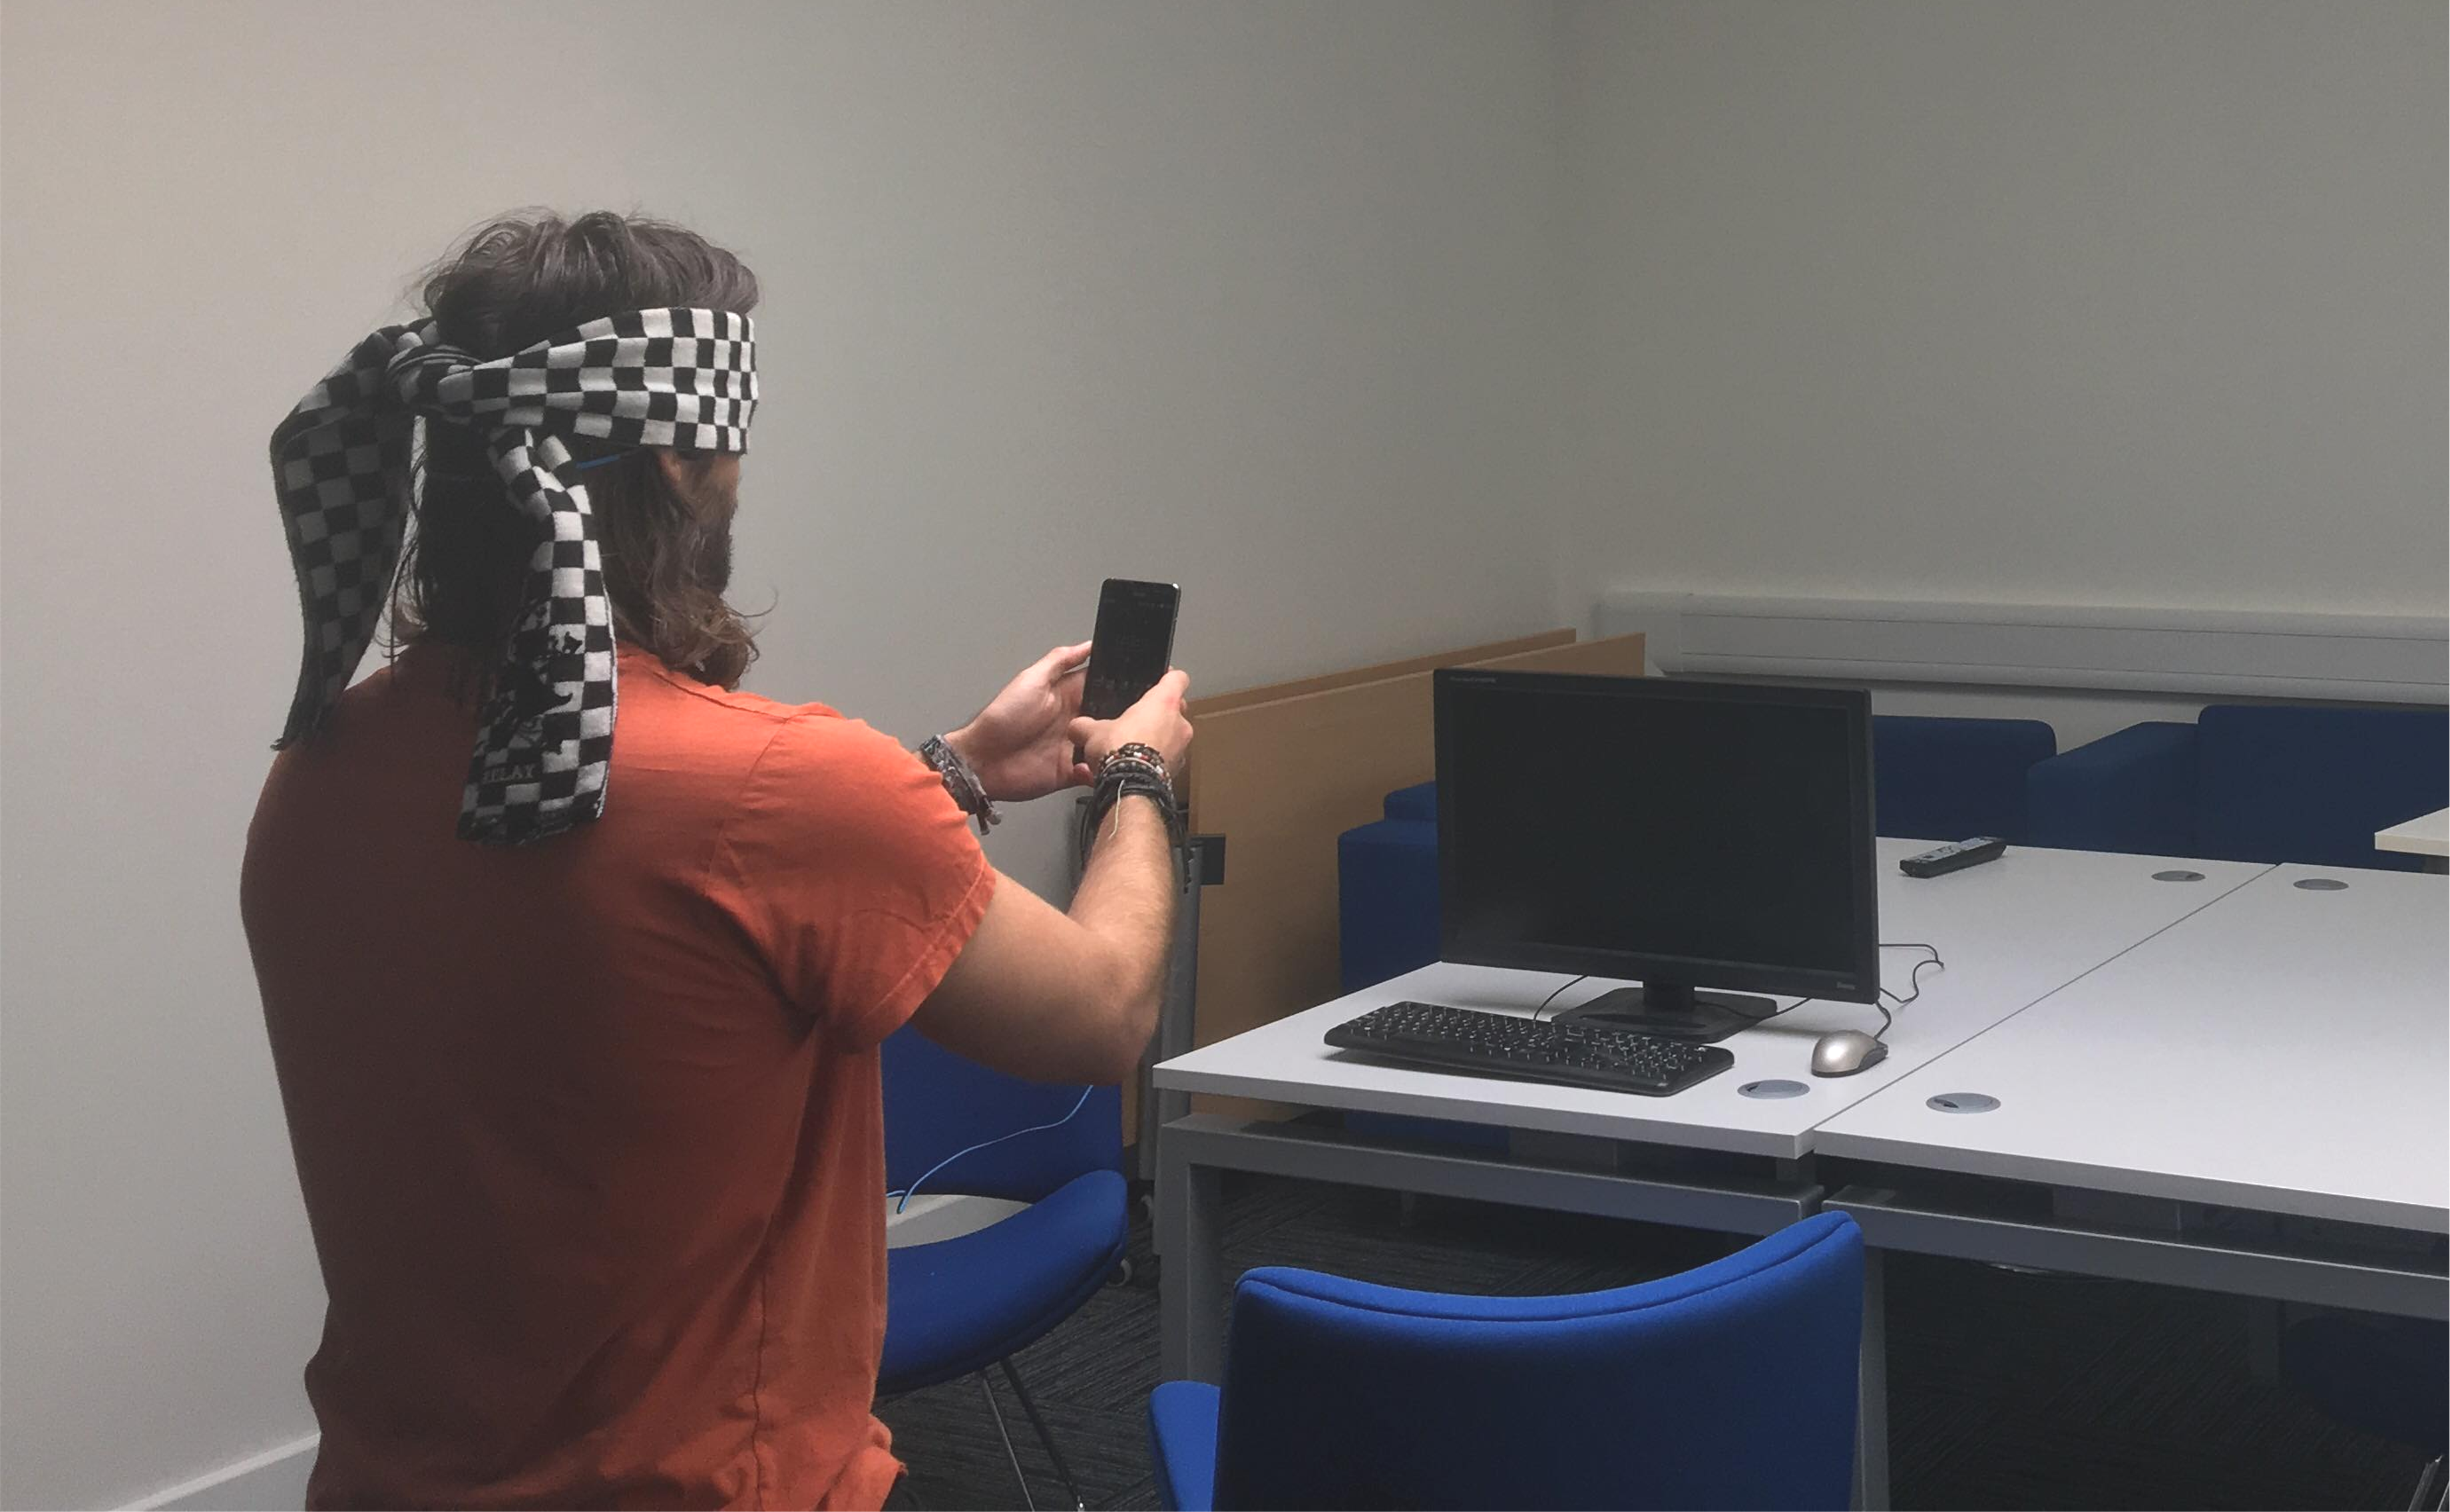
\includegraphics[height=4cm]{figures/system_use.png} \hfil
  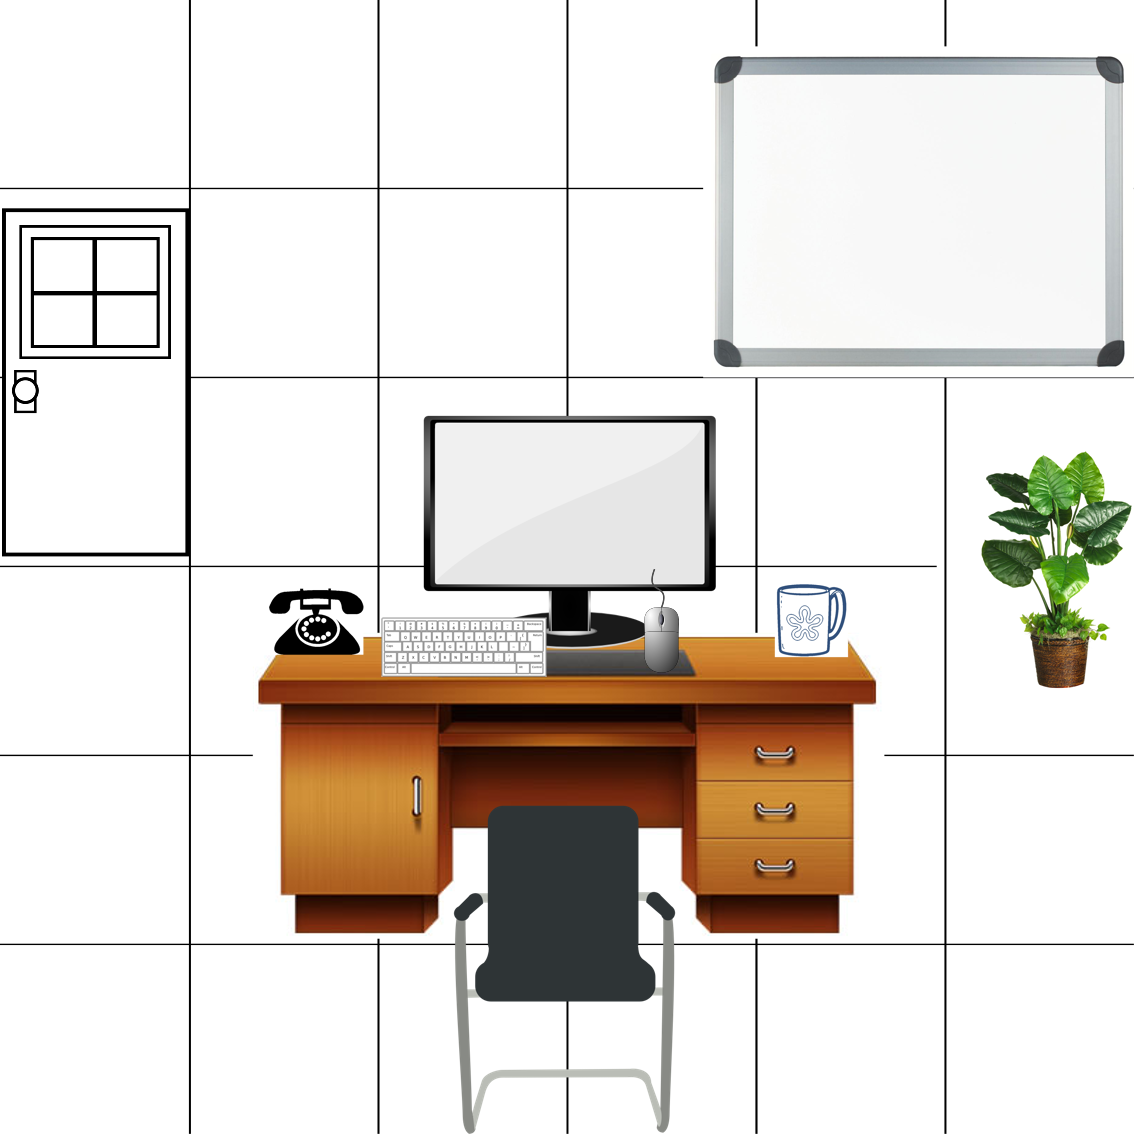
\includegraphics[height=4cm]{figures/object_grid/grid.png}
  \caption{The system in use during an experiment with a blindfolded participant. \tofix{can you add another image with (most of) the objects? maybe arranged in a grid} }\label{fig:system-in-use}
\end{figure}

ActiVis uses the camera's current and previous image data as input and leverages its understanding of inter-object spatial relationships to determine the best navigation action to find the target object.
For this, we expanded upon our previous work and implemented a Partially Observable Markov Decision Process (POMDP) on a mobile phone that generates real-time navigation instructions for the user.
The current paper includes the following main contributions:

\begin{itemize}
  \item a new controller that enables object search and guidance on a mobile phone;
  \item a complete system pipeline that includes audio interface, object detection and human control;
  \item experiments that evaluate the efficacy of the proposed system.
\end{itemize}

Section~\ref{sec:previous-work} discusses relevant previous work, followed by a description of the active vision system and controller in Section~\ref{sec:active-vision}.
The experiments and their results are discussed in Sections~\ref{sec:experiments} and~\ref{sec:results}.
The paper is concluded in Section~\ref{sec:conclusion}.

\section{Previous Work}\label{sec:previous-work}

Early attempts to solve this guidance problem used markers encoded with object or environmental information and a smartphone that scans the environment for these simple patterns~\cite{gude2013blind,manduchi2012mobile}. 
The device uses audio feedback to read out the embedded information or guide the user towards the markers. 
While improvements to feature detectors have made it viable to replace markers with real objects~\cite{redmon2016you}, an alternative guidance approach is proposed in VizWiz~\cite{bigham2010vizwiz} which uses a Mechanical Turk worker to manually locate and guide towards the desired object within a user-provided picture. 

The issue with a marker-based approach is that it requires significant effort to place and maintain them in an environment, which is remedied by markerless systems.
However, both of these methods use passive guidance approaches that rely on the user placing the desired marker/object within the camera's view by themselves before any guidance is provided. 
VizWiz~\cite{bigham2010vizwiz} can leverage a human's understanding of the environment to guide a user to the correct location, but there is significant lag and a reliance on a good internet connection and remote worker being available. 
Previous work on the ActiVis system~\cite{lock2019active} addressed the passive guidance issue by implementing a Markov Decision Process (MDP) that gives the user pointing instructions to find an out-of-view object, showing that this is a viable method for object search. 
However, that work used QR-codes to simulate real objects and on-screen prompts to present the guidance instructions.
In this paper we expand the control model, replacing the QR-codes with real objects and providing audio guidance, thereby implementing a complete object detection and guidance pipeline for people with vision impairments.  

Object detectors can be broadly classified in two-stage models, which use an external algorithm to select regions of interest where to perform object inference~\cite{ren2015faster}, and single-stage models, which generate multiple windows of different sizes and checks each window for any objects.
Between these two classes, there is a speed-accuracy trade-off, where the two-stage models typically produce more accurate results, but are slower and require more computing resources~\cite{liu2018deeplf}.
On the other hand, single-stage models, such as SSD and MobileNet~\cite{liu2016ssd,howard2017mobilenet}, produce less accurate results but require significantly less parameters and FLOPS to perform object inference than the two-stage models. 

\section{Active Vision System}\label{sec:active-vision}

A complete system diagram for ActiVis is given in Fig.~\ref{fig:sys-diagram}. 
This diagram shows a typical feedback control loop that generates a control signal to minimise some error signal, $e$, and drive the output to some reference, $r$. In our case, the system incorporates a human within the loop; $r$ is the target object and $y$ is the actual observation of the mobile phone's camera.

\begin{figure}[t]
  \centering
  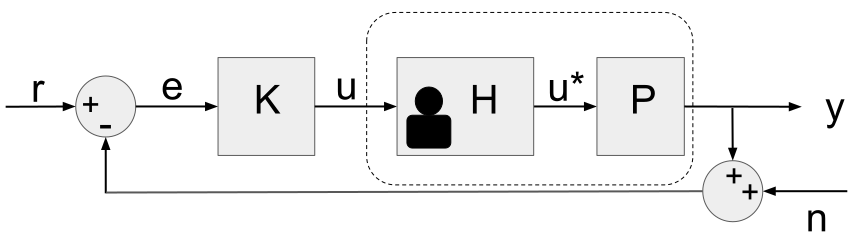
\includegraphics[width=0.7\textwidth]{figures/control_loop.png}
  \caption{The system control loop including a human and the controller.}\label{fig:sys-diagram}
\end{figure}

Adding a human into the loop means to have an additional block, $H$, representing a human that receives a control signal, $u$, from the controller, $K$. 
However, the challenge is that a person may interpret $u$ in some unpredictable way, resulting in the signal $u*$ that points the camera, $P$, to a new object observation,~$y$.
It is therefore important to design $K$ to be robust enough to accommodate different user habits and limitations, ensuring that $u*$ tracks $u$ as closely as possible. 
The object detector's classification errors, $n$, is added to the feedback loop as a noise signal that affects $K$'s output.

In our previous work~\cite{lock2019active}, we assumed a perfect object classifier and solved the problem using an MDP.
In this paper we remove that assumption and replace the MDP with a POMDP-based controller that can handle uncertainties in the object detection and classification. 
Our new controller works by generating a trail of virtual waypoints for the user to point the camera towards, which eventually leads to the target object.
The waypoint positions are based on the model's pre-trained internal knowledge of the inter-object spatial relationships and they are placed in a way that maximises the probability of the user finding the target object.
The design and implementation of this controller are discussed next.

\subsection{Controller Design}

A POMDP is an extension of the MDP that handles cases where the state is not directly observable, allowing it to be used in more realistic scenarios. 
The implication of this is that a POMDP-based agent does not know its state at any point in time, but must infer it based on the known model parameters and sensor accuracy, which in our case is the object detector's accuracy.
This state inference relies on a so-called {\em belief meta-state}, which is updated with additional observations to reflect the likelihood that the agent is in any given state.
The belief state is fully observable by the agent and can be used to infer the mobile device's current state and generate the next action.

A POMDP model is described by the 8-tuple $(\mathbf{S}, \mathbf{A}, \mathbf{T}, \mathbf{R}, \mathbf{\Omega}, \mathbf{O}, \mathbf{b}, \gamma)$, where $\mathbf{S}$ represents a finite set of discrete states, $\mathbf{A}$ is a set of discrete actions, $\mathbf{T}$ is a matrix containing the probabilities of transitioning from state $s$ to state $s'$ (where $s, s' \in \mathbf{S}$) after executing action $a$ (where $a \in \mathbf{A}$), and $\mathbf{R}$ is the reward the agent receives executing action $a$ and reaching state $s'$.
$\mathbf{\Omega}$ is the set of possible state observations, while the matrix $\mathbf{O}$ contains the probabilities of making observation $o \in \mathbf{\Omega}$ when in state $s$ after executing action $a$. \tofix{sure about this? I think the observation is before the action...}
Finally, $\mathbf{b}$ is the belief vector containing the state probability distribution and $\gamma$ is a discount factor that prioritises long-term over short-term rewards, which affects the model's convergence rate. 
The POMDP's parameters and training process are discussed next. 

\subsubsection{Parameters}

The state is given by $s = \langle u, n, v \rangle$, where $u$ is the object within view, $n$ is the number of search steps taken during the search and $v$ is a binary variable indicating whether a waypoint has been visited or not.

The possible actions that dictates the location where the mobile device will generate the next waypoint are given by $\mathbf{A} = \{ \textrm{UP, DOWN, LEFT, RIGHT} \}$.

$\mathbf{T}$ was determined by extracting the inter-object spatial relationships for a limited number of objects, in terms of the actions $\mathbf{A}$, from the OpenImages~\cite{openimages} dataset. 
For example, by iterating over the images containing the objects of interest, we can see that the object `monitor' is located above (i.e. UP) the object `keyboard' in 16\% of the images containing both objects (see Fig.~\ref{fig:openimage}). 
The transition function for this case is $t(s, a, s') = t(\textrm{keyboard}, \textrm{UP}, \textrm{monitor}) = 0.16$.

\begin{figure}[t]
  \centering
  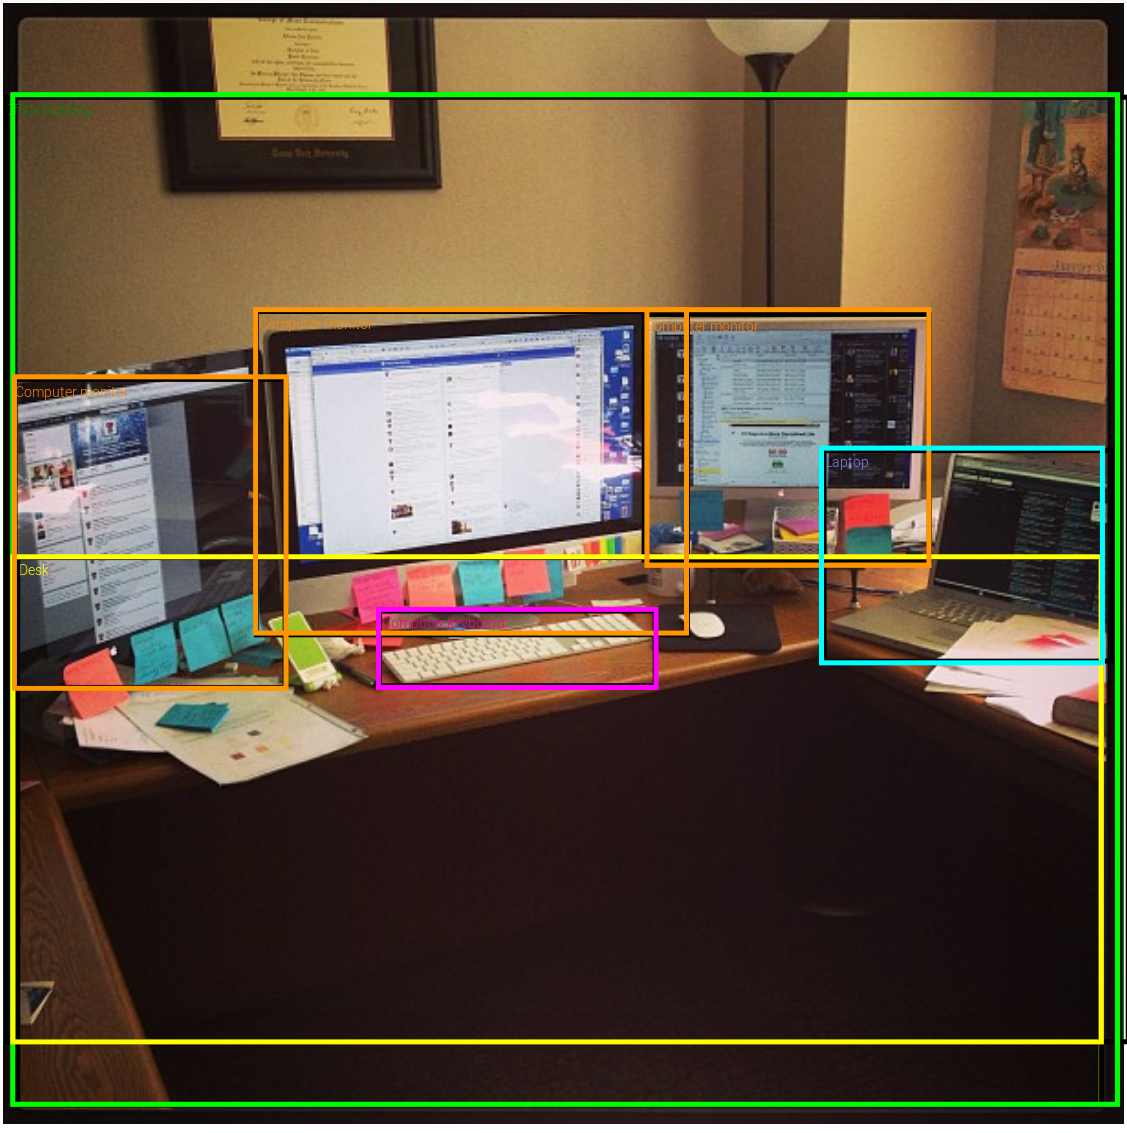
\includegraphics[height=4cm]{figures/desk_example.png} \hfil
  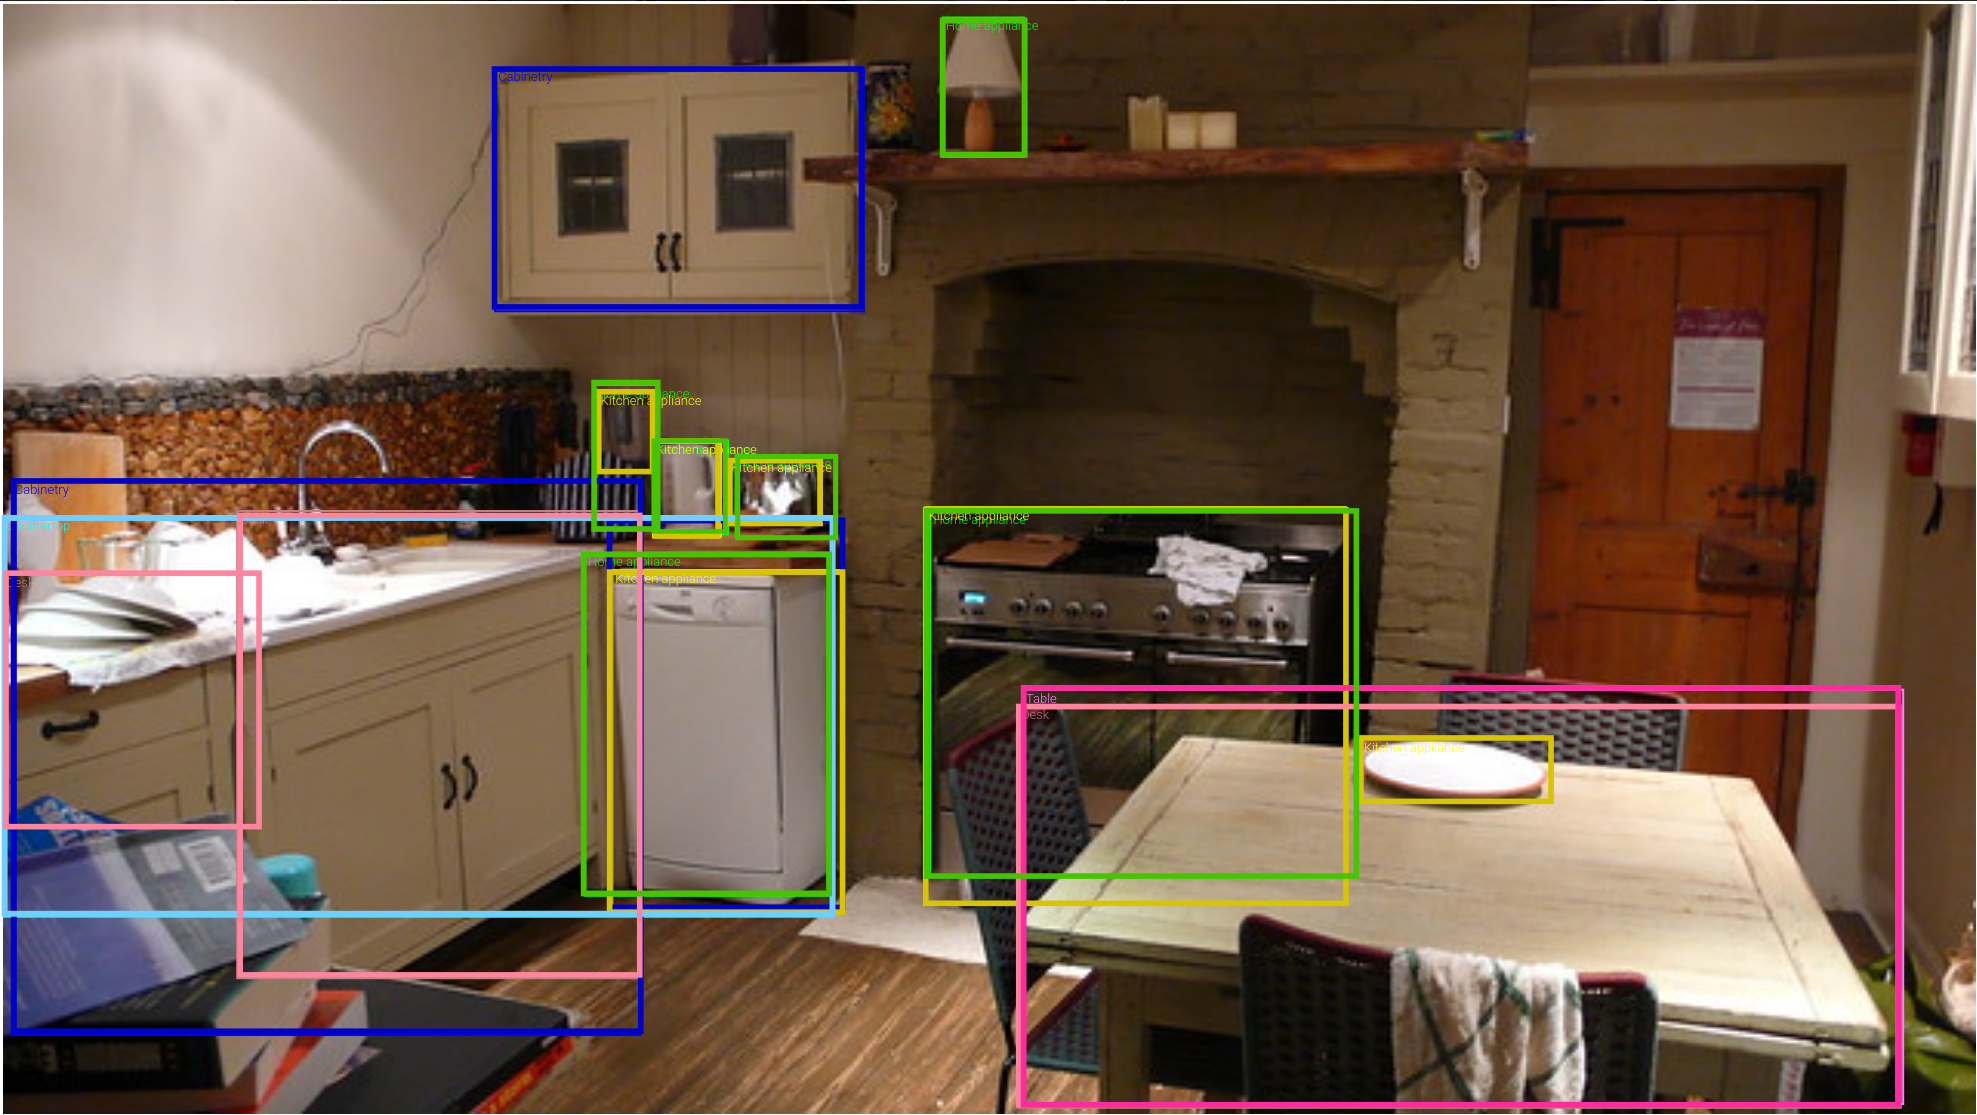
\includegraphics[height=4cm]{figures/kitchen_example_thicc.png}
  \caption{Images from the OpenImage dataset~\cite{openimages} containing some typical objects.}\label{fig:openimage}
\end{figure}

The reward function encourages the device controller to search for the target object by giving a substantial reward if the object is found, while penalising the controller for every action that does not result in a successful object detection.
Furthermore, additional penalties are given if the controller generates a waypoint in an area it has explored before $(v = \textrm{true}$) or when it exceeds some search-length threshold denoted by $n_{\max}$.
The reward values were empirically determined starting from the implementation of our previous MDP model~\cite{lock2019active}, the rewards of which are summarised in Table~\ref{tab:rewards} together with the new ones. \tofix{can you explain why the last reward (otherwise) is much bigger than before, even bigger than the -75 rewards?}

\begin{table}
  \centering
  \caption{The reward function for the POMDP. }\label{tab:rewards}
  \begin{tabular}{p{3cm}p{2cm}p{2cm}}
    \toprule
    Reward condition        & POMDP  & MDP~\cite{lock2019active}   \\ \midrule
    $r(o = o_{target})$     & 10000  & 10000 \\ 
    $r(v = \textrm{true})$  & -75    & -10   \\
    $r(n > n_{\max})$       & -75    & -10   \\
    otherwise $r(\cdot)$    & -100   & -1    \\
    \bottomrule
  \end{tabular}
\end{table}

The state observations are identical to the states that the mobile device can enter into. 
In this case, however, uncertainty is introduced into the observation by the object detector.
Instead, the previous search locations and search time are fully observable, since they can be tracked by the mobile device.
$\mathbf{\Omega}$ therefore only contains the classification/misclassification probabilities of the object detector.
These values were found by performing a set of classification tests with the object detector and generating a confusion matrix to populate $\mathbf{\Omega}$. \tofix{you mean $\mathbf{O}$?}

\subsubsection{Training}

We encoded 15+1 objects into the current system, including a `nothing' item in case the detector does not see anything of interest:
\begin{equation*}
  \begin{split}
    \mathbf{U} = \{ nothing, monitor, keyboard, mouse, desk, laptop, mug, window,\\ 
      lamp, backpack, chair, couch, plant, telephone, whiteboard, door \}.
  \end{split}
\end{equation*}

\noindent We set $n_{\max}$ to 11 waypoints, after which the agent gets penalised for every additional waypoint it generates that does not lead to the target object. 
This results in a total of 352 reachable states ($n_{states} = 16\times11\times2$), with any state containing the target object acting as a terminal state.

The POMDP model is trained to generate a policy that contains the optimal belief-action mapping, which the controller can use to produce the optimal waypoint locations.
This is done by the model exploring the entire state-action-observation space and optimising the policy to maximise its long-term cumulative reward.
However, $\mathbf{b}$ is a vector of continuous probability distributions with infinite combinations, making POMDPs time-consuming or even impossible to solve exactly.
This was the case for our moderately-sized state space, so we opted for an approximate method instead, using the Point-Based Value Iteration~(PBVI) algorithm~\cite{pineau2003point} implemented in the AI-Toolbox library\footnote{http://github.com/Svalorzen/AI-Toolbox}.
The PBVI algorithm speeds up the training process by selecting a smaller subset of representative belief points from $\mathbf{b}$ and tracking these points only. 
Using the PBVI algorithm, we generated a total of 15 policies, one for each target object. 

\subsection{Guidance System Implementation}

We implemented the object detector and the POMDP controller in an Android app and combined it with an audio interface that provides non-visual guidance instructions.
We use non-intrusive bone-conducting headphones to transmit the audio signals to the user without blocking other ambient sounds.

\subsubsection{Audio Interface}
To describe the waypoints' pan and tilt positions, we implemented an improved version of the interface described in~\cite{bellotto2013} that uses a spatialised audio signal.
However, since our headphones bypass the ear's pinnae that allow a person to localise the height~\cite{roffler1968factors}, we spatialise the audio in the pan dimension only.
To convey the tilt angle, we instead exploit a human's natural association of high and low sound sources with a high and low sound frequency, respectively~\cite{blauert1997spatial}, and adjust the sound source's pitch accordingly. 
A similar approach was used in~\cite{schauerte2012assistive}.

\subsubsection{Object Detector}
To recognise objects we used SSD-Lite, which is a single-stage object detection and classification network based on the SSD architecture that implements MobileNetV2~\cite{sandler2018mobilenetv2}.
This is a lightweight model that requires relatively little memory to perform inference tasks, making it suitable for mobile platforms. 
This model achieves a mean average precision~(mAP) of 0.22 with 4.3M parameters and 0.8B~FLOPS on the COCO dataset~\cite{li2018tinydsod}.
The full SSD model achieves a slightly higher mAP (0.25), but with significantly more parameters (34.3M) and FLOPS (34.36B).

The network was trained with a maximum of 10,000 object samples for each class in $\mathbf{U}$, taken from the OpenImages dataset~\cite{openimages}, with a 60-20-20\% split for training, validation and testing respectively.
We set a relatively high confidence threshold of 0.7 to reduce the likelihood of false-positives.
Training for 120 epochs, with 1000 iterations each, we achieved a mAP of 0.16 on this dataset and produced a TensorFlow Lite model that is Android-compatible. We used this model to finally implement our SSD-Lite object detector on the mobile device.

\subsubsection{Waypoint Generation}
To search the target object, the system uses the policy file from the POMDP training process, which defines the best location of next waypoint based on the device's current state.
This state is tracked by the device throughout the app's runtime by performing object detection and recording the previous search locations and waypoint positions.
The latter are obtained by discretising the world into a $6\times6$ grid, where each cell represents a \SI{35}{\degree} rotation, and setting the relevant grid unit's $v$ value when visited.
This setup gives the state access to perfectly observable $n$ and $v$ parameters, while the observation $o$ is generated by the object detector. 
When the device makes a new observation, either because the user rotates the device past \SI{35}{\degree} or sees a new object, the device triggers the controller to generate a new waypoint location.
The controller uses $o$ to update $\mathbf{b}$ and queries the policy for the best location to place the new waypoint. 
The policy output is an action from $\mathbf{A}$ that indicates the next adjacent grid square to place the waypoint, e.g. an `UP' output would result in a waypoint being placed one grid square above the current view. 
\tofix{double-check all the quantities an definitions in this section (i.e. states, observations, etc.) are correct, because some were a little mixed-up...}


\section{Experiment Design}\label{sec:experiments}

To evaluate the guidance system's effectiveness, we designed a set of experiments to measure its performance in driving a user towards a target object within a static environment. 
We conducted an additional set of experiments with an alternative system that relies on a user's intuition and prior knowledge to generate actions instead, to act as a baseline measurement for our system's results. 

Both experiment environments and the object placements within them were modelled on a typical office and care was taken to ensure that both environments were unique in layout and object placement, though some cross-experiment occurrences appear with the larger, more static objects. 
To minimise any cross-experiment learning effects, 2 different sets of objects were used for each experiment and any objects that occurred in both experiments were placed at different positions for each experiment. 
The objects in the guided experiment environment are $\mathbf{u}_{guided} = \{ door$, $desk$, $chair$, $whiteboard$, $mouse$, $laptop$, $backpack$, $mug \}$, while the objects in the unguided experiment are $\mathbf{u}_{unguided} = \{ door$, $desk$, $chair$, $whiteboard$, $mouse$, $monitor$, $telephone$, $keyboard \}$.

We recruited 10 participants (8 male, 2 female; average age 29.2 years) for the experiments, including 2 legally blind participants. 
The other 8 participants were blindfolded to simulate blindness. 
The app was run on an Asus ZenPhone AR with Android 7.0 and ARCore\footnote{http://developers.google.com/ar/} and text-to-speech enabled. 
A time limit of 45 seconds was set for each experiment run, which was ended when the target object was found or the time limit was reached, and there was one experiment run per target in the respective environment.

\subsection{Unguided Case}

The goal of this experiment is to mimic a typical person with healthy eyesight's search behaviour. 
In such a scenario, a person would see the objects currently within their field of view and use their prior knowledge and intuition to make a decision on where to look next.
For example, a person in bathroom facing the basin after washing their hands is unlikely to find a hand dryer placed above or below the basin so it is reasonable to believe that they would instinctively look at chest height on the walls to their left, right or behind them instead. 

For this experiment, the mobile camera and object detector acts as the participants' eyes and informs them about the objects within the camera's view.
It is then up to the participant to exploit their prior knowledge and intuition to manipulate the camera and find the target object. 
In this case, the human acts as both the controller and actuator. 
The app only reads out the objects upon the user's request by tapping on the screen. 
When the target object comes within the camera's view and is correctly detected, the device vibrates to inform the participant. 

To mimic the normal search behaviour and allow the participant's to use their intuition and prior knowledge, we ignored the learning effect for this experiment and verbally informed them what their target was for each experiment run.

\subsection{Guided Case}

In this experiment, we evaluate the performance of the guidance system in an object search task, where the perception and control tasks are performed by the guidance system and the participant acts as the actuator, interpreting control signals and outputting actuation forces on the camera sensor. 
This is modelled in the schematic in Fig.~\ref{fig:sys-diagram}. 

The participants were not told what the targets objects were in this experiment to eliminate the possibility of them ignoring the guidance instructions in order to try and find the target object faster themselves.
This also isolated the performance measurement to the guidance system alone.
An experiment run started with the experiment staff selecting the target.

\section{Results}\label{sec:results}

\subsection{Target Acquisition}

The target acquisition rate (TAR) is the proportion of objects the participants found during an experiment. 
For example, a TAR of 0.5 indicates that a participant found the target object in 50\% of searches. 
Taking each participant's TAR as a datum, we found the unguided case produced a higher average TAR (0.54 vs. 0.46), meaning that participants found 8\% more objects without guidance instructions.
However, the Kruskal-Wallis (KW) test for non-normal data shows that these results are statistically not significantly different ($p_{kw} = 0.16$), meaning we cannot conclude which experiment produced the best TAR. 
All the experiment results are summarised in Table~\ref{tab:results}. 

\begin{table}
  \centering
  \caption{A summary of the experiment results. }\label{tab:results}
  \begin{tabular}{p{5cm}p{2cm}p{2cm}p{2.5cm}}
    \toprule
    & \textbf{Guided}             & \textbf{Unguided} & \textbf{KW Statistic} \\\midrule
    TAR [\%]                      & $46\pm13$         & $54\pm15$     &  0.16 \\\midrule
    Time to target [s]            & $12.5\pm11.9$     & $17.2\pm11.5$ & 0.045 \\\midrule
    Pan Angle Displacement [rad]  & $0.68\pm1.1$      & $0.99\pm1.2$  & 0.029 \\\midrule
    Tilt Angle Displacement [rad] & $0.68\pm1.1$      & $1.04\pm1.2$  & 0.011 \\\midrule
    Linear Displacement [rad]     & $0.23\pm0.22$     & $0.36\pm0.22$ & 0.012 \\\midrule
    \bottomrule
  \end{tabular}
\end{table}

\subsection{Time to Target}

The time it takes to find a target object is an important indicator of system performance, where less time indicates a shorter search time and increased performance.
The data for the search times for each experiment are shown in Fig.~\ref{fig:boxplots}.

\begin{figure}[t]
  \centering
  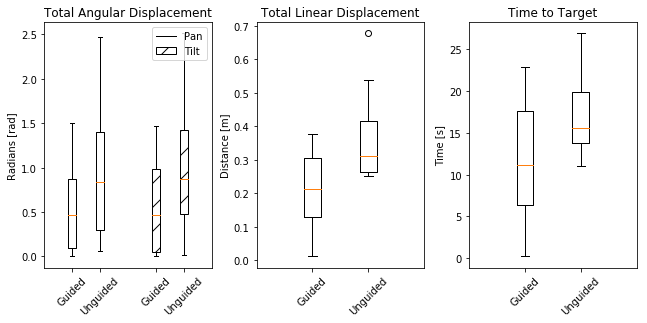
\includegraphics[width=1.0\textwidth]{figures/boxplot_combined.png}
  \caption{A set of boxplots comparing the total linear and angular displacements, as well as the time to target for each experiment. }\label{fig:boxplots}
\end{figure}

From Fig.~\ref{fig:boxplots}, it can be seen that the guidance system reduced the overall time it took the participants to find each target object.
This is confirmed by the data that show an average search time of 12.5s for the guided experiment and 17.2s for the unguided case ($p_{kw}=0.045$), an improvement of around 27\%.
These results compare favourably with those collected from experiments performed with this system's previous iteration where an average time to target of 31s was recorded~\cite{lock2019active}. 
However, it should be noted that the system implementation and experiment design for this work is significantly different and this comparison is symbolic more than it is indicative of major improvement.
\todo{How to relate the VISAPP work to these results? The experiments are different, so the data aren't directly comparable.}

\subsection{Movement}

To give an indication of the effort required to find each target, we look at the mobile device's displacement data. 
In this case, less device displacement is desirable, since it implies less physical exertion was demanded from the user.

The device displacement was measured in both linear ($x, y, z$) and angular (pan, tilt) dimensions.
Integrating these data, we obtain the total absolute displacement in each dimension.
These results are plotted in Fig.~\ref{fig:boxplots}.

%\begin{figure}[t]
  %\centering
  %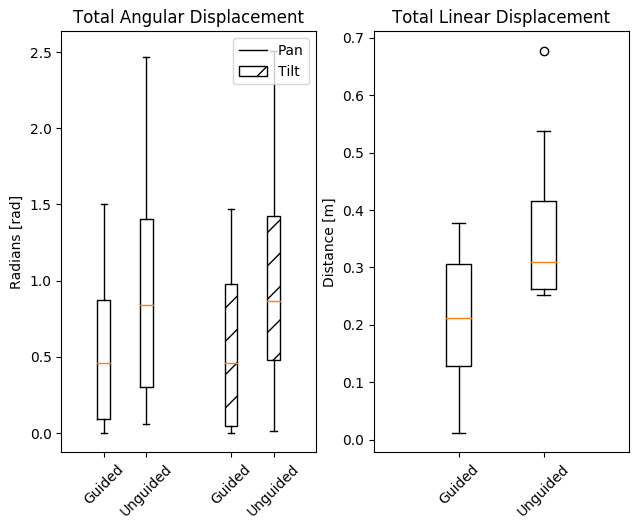
\includegraphics[width=0.6\textwidth]{figures/boxplot_displacement.png}
  %\caption{A set of boxplots comparing the linear and angular displacement the device travelled for each experiment.\tofix{Half the height of the image. You can also put it together with Fig.~4 to save space.}}\label{fig:boxplot-displacement}
%\end{figure}

The boxplots for the total angle displacement show a consistent reduction in radians for the guided case for both the pan (\SI{0.68}{\radian} vs. \SI{0.99}{\radian}, $p_{kw}=0.029$) and tilt dimensions (\SI{0.68}{\radian} vs. \SI{1.05}{\radian}, $p_{kw}=0.011$). 
The guidance system therefore reduces the total angular displacement to find the objects by 31\% and 35\% for the pan and tilt dimensions respectively. 
The total linear displacement is also reduced when using the guidance interface by approximately 36\% (\SI{0.23}{\metre} vs. \SI{0.36}{\metre}, $p_{kw}=0.012$).
These results are summarised in Table~\ref{tab:results}.
To conclude, the data show that the guidance interface reduced the total angular and linear displacement required to find the target objects in all dimensions by at least 31\%, reducing the total effort required by the user. 

\todo{Make sure paper fits into 10+1 page limit for content and references}

\section{Conclusion}\label{sec:conclusion}

In this work, we presented ActiVis, a mobile guidance system that uses an object detector to scan the environment for objects and a POMDP-based controller and audio interface to generate and present the user with guidance instructions. 
We implemented this system on an Android app and tested it with a group of 10 participants to evaluate its effectiveness compared to a baseline, unguided case that only uses the object detector and relies on the human to generate the search path. 
The key results from these experiments are that the guidance system improved the participants' target-searching performance, reducing the total search time and overall camera manipulation effort required when compared to a base case.
However, the participants were able to find 8\% more objects on average in the unguided case, but this result was found to be statistically insignificant. 
With these results, we can reasonably conclude that our system enables a blind or blindfolded user to find a target object and does so better than the alternative base case.

The next steps for the project are to refine and expand the object detector to include objects from other environments. \tofix{that's it? a little bit more imagination... what about user- adaptation? different interface, maybe with different audio, voice, vibration etc.? evaluation with larger pool of VI participants? It doesn't mean you have to do it, but it gives ideas for future improvements and research projects.}

\paragraph{{\bf Acknowledgements.}}\label{sec:acknowledge}
This research is partly supported by a Google Faculty Research Award (Winter 2015).
\tofix{any charity directly involved in the experiments?}

\tofix{check all references to use correct information and full list of authors (suggest to use manual input on tools like JabRef)}
\bibliographystyle{splncs04}
\bibliography{bib}

\end{document}
